\documentclass[tikz,border=5pt]{standalone}
\usepackage[T1]{fontenc}
\usepackage{lmodern,amsmath,amssymb}
\usetikzlibrary{arrows.meta,calc,positioning,fit,backgrounds,shapes.geometric,matrix,decorations.pathreplacing,patterns}
\definecolor{ink}{gray}{0.08}
\definecolor{wash}{gray}{0.965}
\definecolor{soft}{gray}{0.45}
\tikzset{box/.style={draw=ink,line width=.65pt,fill=white,align=center,inner sep=4pt,outer sep=0pt,font=\small},flow/.style={draw=ink,line width=.65pt,-{Latex[length=1.8mm,width=1.3mm]},rounded corners=2pt},annotation/.style={font=\scriptsize,text=soft,align=center},groupbox/.style={draw=soft,dashed,line width=.45pt,fill=wash}}
\begin{document}
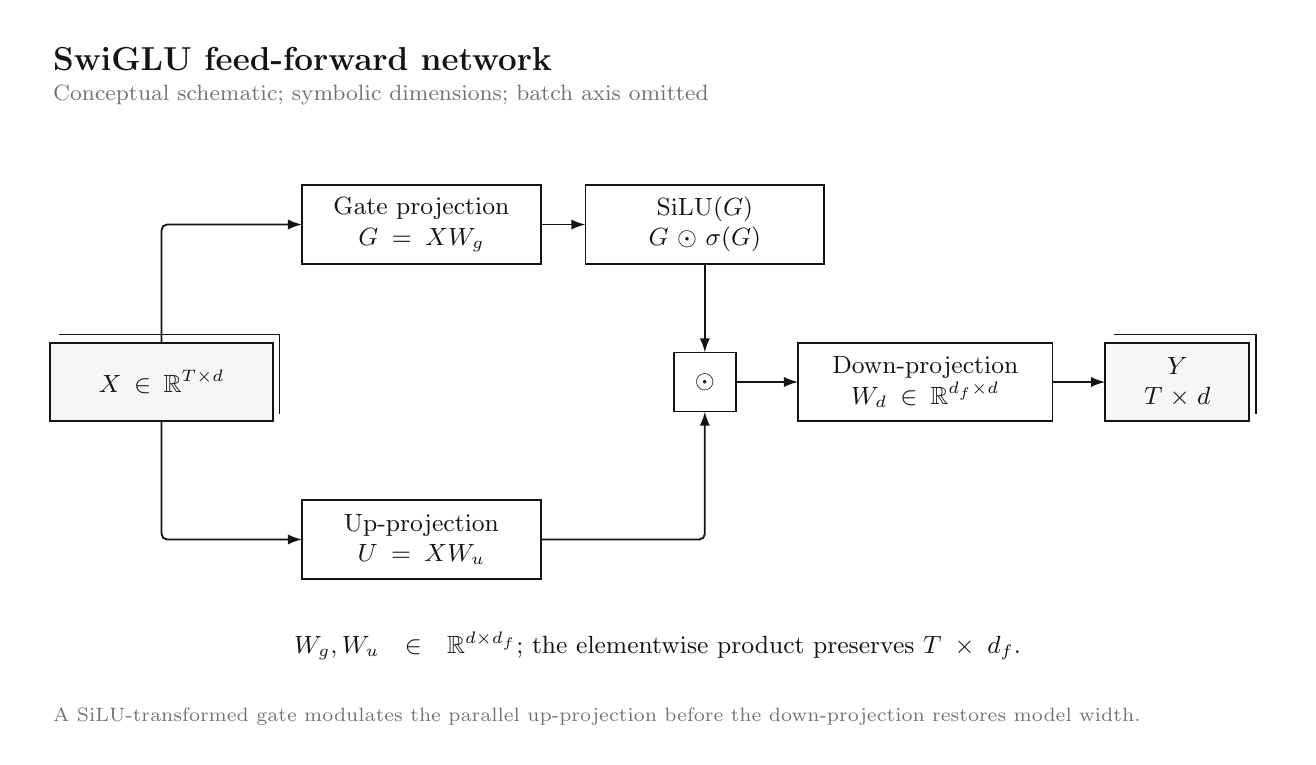
\begin{tikzpicture}[x=1cm,y=-1cm,font=\rmfamily,text=ink]

\path[use as bounding box] (0,0) rectangle (16,9);
\node[anchor=west,font=\large\bfseries] at (.2,.4) {SwiGLU feed-forward network};
\node[anchor=west,font=\footnotesize,text=soft] at (.2,.85) {Conceptual schematic; symbolic dimensions; batch axis omitted};
\begin{pgfonlayer}{background}
\end{pgfonlayer}
\node[box,fill=wash,minimum width=2.8cm,minimum height=1.0cm,text width=2.55cm] (x) at (1.7,4.5) {$X\in\mathbb{R}^{T\times d}$};
\draw[ink,line width=.4pt] (0.4,3.9) -- (3.1999999999999997,3.9) -- (3.1999999999999997,4.9);
\node[box,minimum width=3.0cm,minimum height=1.0cm,text width=2.75cm] (wg) at (5.0,2.5) {Gate projection\\$G=XW_g$};
\node[box,minimum width=3.0cm,minimum height=1.0cm,text width=2.75cm] (wu) at (5.0,6.5) {Up-projection\\$U=XW_u$};
\node[box,minimum width=3.0cm,minimum height=1.0cm,text width=2.75cm] (silu) at (8.6,2.5) {$\operatorname{SiLU}(G)$\\$G\odot\sigma(G)$};
\node[box,minimum width=0.75cm,minimum height=0.75cm,text width=0.5cm] (mul) at (8.6,4.5) {$\odot$};
\node[box,minimum width=3.2cm,minimum height=1.0cm,text width=2.95cm] (wd) at (11.4,4.5) {Down-projection\\$W_d\in\mathbb{R}^{d_f\times d}$};
\node[box,fill=wash,minimum width=1.8cm,minimum height=1.0cm,text width=1.55cm] (out) at (14.6,4.5) {$Y$\\$T\times d$};
\draw[ink,line width=.4pt] (13.799999999999999,3.9) -- (15.6,3.9) -- (15.6,4.9);
\node[align=center,inner sep=0pt,outer sep=0pt,font=\small,minimum width=12.8cm,minimum height=0.6cm,text width=12.55cm] (note7) at (8,7.85) {$W_g,W_u\in\mathbb{R}^{d\times d_f}$; the elementwise product preserves $T\times d_f$.};
\begin{pgfonlayer}{background}
\draw[flow] (x.north) -- (1.7,2.5) -- (wg.west);
\draw[flow] (x.south) -- (1.7,6.5) -- (wu.west);
\draw[flow] (wg.east) -- (silu.west);
\draw[flow] (silu.south) -- (mul.north);
\draw[flow] (wu.east) -- (8.6,6.5) -- (mul.south);
\draw[flow] (mul.east) -- (wd.west);
\draw[flow] (wd.east) -- (out.west);
\end{pgfonlayer}
\node[anchor=west,align=left,font=\scriptsize,text=soft,text width=15.6cm] at (.2,8.75) {A SiLU-transformed gate modulates the parallel up-projection before the down-projection restores model width.};
\end{tikzpicture}
\end{document}
